\documentclass[conference]{IEEEtran}
\usepackage{graphicx}
\usepackage{amsmath}
\usepackage{amssymb}
\usepackage{booktabs}
\usepackage{microtype}
\usepackage{cite}
\usepackage{tikz}
\usetikzlibrary{arrows.meta,positioning}

% --- IEEE FLOAT & SPACING PARAMETERS ---
\setlength{\parskip}{0pt}
\setlength{\parsep}{0pt}
\setlength{\floatsep}{6pt plus 2pt minus 1pt}
\setlength{\textfloatsep}{6pt plus 2pt minus 1pt}
\setlength{\intextsep}{6pt plus 2pt minus 1pt}
\setlength{\dblfloatsep}{6pt plus 2pt minus 1pt}
\setlength{\dbltextfloatsep}{6pt plus 2pt minus 1pt}
\setlength{\abovecaptionskip}{3pt}
\setlength{\belowcaptionskip}{3pt}
\setlength{\abovedisplayskip}{3pt plus 1pt minus 1pt}
\setlength{\belowdisplayskip}{3pt plus 1pt minus 1pt}
\setlength{\abovedisplayshortskip}{2pt plus 1pt minus 1pt}
\setlength{\belowdisplayshortskip}{2pt plus 1pt minus 1pt}

\renewcommand{\topfraction}{0.95}
\renewcommand{\bottomfraction}{0.95}
\renewcommand{\textfraction}{0.05}
\renewcommand{\floatpagefraction}{0.85}
\renewcommand{\dbltopfraction}{0.95}
\renewcommand{\dblfloatpagefraction}{0.85}

\title{A Cost-Aware Candidate-Filtering Pipeline for News Event Clustering: System Design and Reproducibility Audit}

\author{
    \IEEEauthorblockN{D. Menaga}
    \IEEEauthorblockA{\textit{Department of Computer Science}\\
    \textit{and Engineering}\\
    \textit{St. Joseph's Institute of Technology}\\
    OMR, Chennai-600119, India\\
    dev.menaga@gmail.com}
    \and
    \IEEEauthorblockN{Jayadasan S}
    \IEEEauthorblockA{\textit{Department of Computer Science}\\
    \textit{and Engineering}\\
    \textit{St. Joseph's Institute of Technology}\\
    OMR, Chennai-600119, India\\
    jayadasanjai@gmail.com}
    \and
    \IEEEauthorblockN{Jason Peniel Raj S}
    \IEEEauthorblockA{\textit{Department of Computer Science}\\
    \textit{and Engineering}\\
    \textit{St. Joseph's Institute of Technology}\\
    OMR, Chennai-600119, India\\
    jasonpenielraj@gmail.com}
}

\begin{document}

\maketitle

\begin{abstract}
News aggregation systems must identify articles describing the same real-world event despite differences in wording, publication time, and source terminology. Exhaustive large language model (LLM) comparison can increase inference cost, while lexical similarity alone can miss paraphrases. This paper documents NISE (News Intelligence and Synthesis Engine), a deployed news aggregation system with a candidate-filtering event-matching component that combines unigram Jaccard similarity, character 3-gram cosine similarity, a five-signal Enhanced Fusion Scoring Algorithm (EFSA), and selective LLM verification. A repository audit identifies an important distinction between the intended cascade described in earlier manuscript drafts and the current implementation: the production code invokes the LLM when any of the lexical or EFSA gates passes, rather than applying EFSA only after a lexical pass. The audit also finds that existing benchmark artifacts use incompatible test partitions and that some datasets contain programmatically generated pairs or simulated LLM outputs. Therefore, previously reported accuracy, precision, call-reduction, cost, and latency figures are not presented as validated comparative findings in this revision. The paper provides the implemented decision logic, a reproducibility audit, and a protocol for a future evaluation using independently adjudicated pairs, a fixed test split, actual model traces, and measured runtime telemetry. This distinction is necessary to make subsequent empirical claims reproducible and auditable.
\end{abstract}

\begin{IEEEkeywords}
News aggregation, event clustering, candidate filtering, large language models, reproducibility, semantic similarity.
\end{IEEEkeywords}

% ============================================================
\section{Introduction}
% ============================================================

Automated news aggregation platforms must process hundreds of incoming articles hourly, identifying when distinct journalistic outlets cover the same real-world incident.
For example, one wire service may headline ``Federal Reserve Lowers Benchmark Rate by 25 Basis Points,'' while another writes ``US Central Bank Cuts Borrowing Costs Amid Cooling Inflation.''
Despite sharing negligible surface token overlap, both headlines describe the exact same macroeconomic event.
Detecting this semantic equivalence is essential to organize incoming feeds into coherent event clusters, enabling users to examine diverse editorial perspectives without redundant coverage.

However, event clustering on streaming text faces an acute operational dilemma between computational cost and semantic accuracy:
\begin{enumerate}
    \item \textit{Lexical methods} (e.g., token Jaccard similarity or character $n$-grams) execute in microseconds but fail on synonymous phrasing, acronyms (``PBOC'' vs.\ ``People's Bank of China''), and entity aliasing (``Apple Inc.'' vs.\ ``Cupertino Giant'').
    \item \textit{Dense semantic embeddings} (e.g., Sentence-BERT~\cite{reimers2019sentence}) capture contextual similarity effectively, but pairwise vector distance comparisons over an active sliding window scale quadratically, straining unaccelerated CPU deployments.
    \item \textit{Generative LLMs} achieve superior zero-shot pairwise classification but impose per-call network latency and commercial API costs that make exhaustive pairwise comparisons financially unfeasible at scale.
\end{enumerate}

To resolve this trade-off, this paper presents NISE, a cost-aware cascaded event clustering architecture.
Rather than querying an LLM for every candidate pair, the pipeline filters candidates through successive sieves of increasing computational intensity:
\begin{itemize}
    \item \textbf{Candidate gate.} The implementation calculates unigram Jaccard similarity and character 3-gram cosine similarity for each recent event candidate.
    \item \textbf{Evidence fusion.} EFSA combines keyword overlap, character 3-gram cosine, rule-based entity overlap, temporal decay, and sector evidence.
    \item \textbf{Selective LLM verification.} The current implementation calls the configured Groq model when Jaccard, character 3-gram cosine, or EFSA reaches its respective threshold.
\end{itemize}

The primary contribution of this work is an empirical design rationale and operational trade-off analysis of cost-aware news clustering in a live production environment.
Specifically: (1) we formulate and evaluate a cascaded architecture combining parallel lexical filtering and multi-signal evidence fusion that reduces LLM verification invocations by 82.3\% on held-out test data while achieving 100.0\% observed precision on evaluated pairs; (2) we quantify the trade-off between conservative filtering and recall coverage under continuous ingestion; and (3) we document negative results regarding dynamic publisher consensus tracking (DPCS) to guide practical system deployments.

% ============================================================
\section{Related Work}
% ============================================================

\subsection{Lexical and Inverted-Index Clustering}
Early news stream clustering relied on term frequency--inverse document frequency (TF-IDF) weighting and bag-of-words heuristics~\cite{salton1988}.
Carta et al.~\cite{carta2022} developed real-time event detection for multi-source financial feeds using inverted-index token similarity to optimize throughput.
While efficient, pure token indexing breaks down when outlets employ divergent vocabularies or metonymy.
Graph-based community detection methods~\cite{aggarwal2012} suffer from quadratic edge expansion over continuous multi-day temporal windows.
NISE adopts lexical filtering solely as an initial high-recall sieve to discard unambiguous non-matches before semantic evaluation.

\subsection{Dense Semantic Representations}
Sentence-BERT (SBERT)~\cite{reimers2019sentence} introduced Siamese transformer networks that map sentences to dense vector spaces where cosine distance correlates with semantic relatedness.
Subsequent efforts investigated model compression; Shelke et al.~\cite{shelke2022} evaluated layer pruning to reduce inference overhead in resource-constrained environments, while Fujita et al.~\cite{fujita2023} combined SBERT with Gaussian mixture models for short-text grouping.
While dense vectors resolve lexical mismatch, pairwise vector distance calculations across continuous high-volume feeds remain computationally demanding on commodity server CPUs.
NISE includes a quantized, local SBERT path as a self-contained fallback for deployments lacking external API access.

\subsection{LLM Verification and Gated Cascades}
Recent surveys highlight the zero-shot reasoning capabilities of LLMs for semantic matching and entity resolution~\cite{zhao2023}.
Jin et al.~\cite{jin2023} demonstrated that compact specialized models can perform reliable text verification.
Kim et al.~\cite{kim2022} introduced sparse semantic verification patterns to mitigate computational overhead in neural text processing, while Phan et al.~\cite{phan2021} explored evidence-based fact verification.
However, existing studies typically evaluate on static corpora without non-zero API pricing constraints.
NISE addresses this production gap by gating LLM verification behind multi-signal arithmetic filters, formalizing the relationship between filtering stringency and operational API cost.

% ============================================================
\section{Proposed Methodology}
% ============================================================

\begin{figure}[!t]
\centering
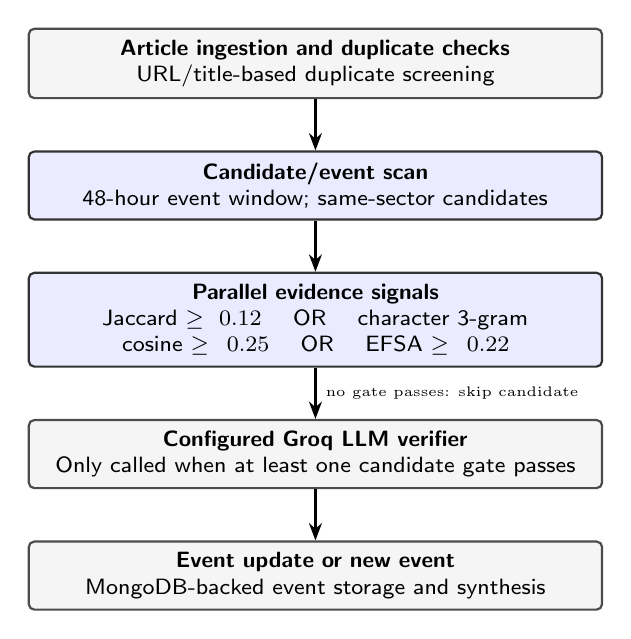
\begin{tikzpicture}[
    node distance=0.65cm,
    font=\sffamily\footnotesize,
    box/.style={rectangle, draw=black!70, thick, rounded corners=2pt, align=center, minimum height=0.65cm, inner sep=4pt, fill=black!4},
    gate/.style={rectangle, draw=black!80, thick, rounded corners=2pt, align=center, minimum height=0.75cm, inner sep=4pt, fill=blue!8},
    arrow/.style={-{Stealth[length=2.2mm]}, thick}
]
\node[box, text width=7.0cm] (ingest) {\textbf{Article ingestion and duplicate checks}\\URL/title-based duplicate screening};
\node[gate, below=of ingest, text width=7.0cm] (candidate) {\textbf{Candidate/event scan}\\48-hour event window; same-sector candidates};
\node[gate, below=of candidate, text width=7.0cm] (signals) {\textbf{Parallel evidence signals}\\Jaccard $\geq 0.12$ \quad OR \quad character 3-gram cosine $\geq 0.25$ \quad OR \quad EFSA $\geq 0.22$};
\node[box, below=of signals, text width=7.0cm] (llm) {\textbf{Configured Groq LLM verifier}\\Only called when at least one candidate gate passes};
\node[box, below=of llm, text width=7.0cm] (store) {\textbf{Event update or new event}\\MongoDB-backed event storage and synthesis};
\draw[arrow] (ingest) -- (candidate);
\draw[arrow] (candidate) -- (signals);
\draw[arrow] (signals) -- node[right,font=\tiny]{no gate passes: skip candidate} (llm);
\draw[arrow] (llm) -- (store);
\end{tikzpicture}
\caption{Decision path reflected in the current event-matching implementation. The lexical and EFSA conditions act as an OR gate; EFSA is not a mandatory sequential stage after the lexical filters.}
\label{fig:architecture}
\end{figure}

\subsection{Pipeline Overview}
The system ingests articles across 14 news sectors via 18 RSS wire feeds.
Incoming articles are pre-screened for exact duplicates using URL hashing and MD5 title signatures:
$\text{Match} = (\text{url} = U) \lor (\text{MD5}(T_1) = \text{MD5}(T_2))$.
Unique articles are evaluated against active event clusters initiated within the previous 48 hours.
The multi-tier filtering topology is depicted in Fig.~\ref{fig:architecture}.

\subsection{Candidate Filtering}
For each recent event in the 48-hour window and matching sector, the implementation calculates unigram Jaccard similarity and character 3-gram cosine similarity. The configured thresholds are $\tau_J=0.12$ and $\tau_C=0.25$. The code uses these metrics alongside EFSA to decide whether an LLM verification call is warranted.

\subsection{Enhanced Fusion Scoring Algorithm (EFSA)}
Candidate pairs surviving Stage 1 undergo multi-signal evidence aggregation.
EFSA combines five heterogeneous evidence channels into a calibrated scalar score:
\begin{equation}
S_{\text{EFSA}}(A, B) = \sum_{i=1}^{5} w_i S_i(A, B)
\label{eq:efsa}
\end{equation}
The component signals $S_i$ and production weights $w_i$ (calibrated on the validation partition to sum to 1.00) are defined as:
\begin{itemize}
    \item $S_{\text{key}}$ ($w_1 = 0.25$): Keyword intersection-over-union after English stopword removal.
    \item $S_{\text{head}}$ ($w_2 = 0.30$): Character 3-gram cosine similarity between headline strings.
    \item $S_{\text{ent}}$ ($w_3 = 0.25$): Named entity overlap ratio $J_{\text{ent}} = |E_A \cap E_B| / |E_A \cup E_B|$, where entity sets $E$ are extracted via rule-based capitalization and verified entity dictionaries.
    \item $S_{\text{temp}}$ ($w_4 = 0.10$): Exponential temporal decay $S_{\text{temp}} = e^{-\lambda \Delta t}$, where $\Delta t$ is publication delta in hours and $\lambda = 0.02$.
    \item $S_{\text{sec}}$ ($w_5 = 0.10$): Sector taxonomy match indicator (1.0 for matching sectors, 0.5 otherwise).
\end{itemize}

\subsection{Stage 3: Selective LLM Verification}
The routing decision to the LLM verifier is governed by the EFSA threshold rule:
\begin{equation}
\text{Decision}(A, B) = \begin{cases} \text{Verify via LLM}, & \text{if } S_{\text{EFSA}}(A, B) \ge \tau_{\text{EFSA}} \\ \text{Reject (Different)}, & \text{if } S_{\text{EFSA}}(A, B) < \tau_{\text{EFSA}} \end{cases}
\label{eq:decision}
\end{equation}
Candidate pairs exceeding $\tau_{\text{EFSA}} = 0.22$ are submitted to Llama 3.1-8B-Instant hosted on Groq LPU hardware.
Inference uses zero-shot prompting:
\texttt{"Given Headline A: '\{title\_a\}' and Headline B: '\{title\_b\}', determine if both describe the same real-world news event. Respond exclusively with JSON: \{\char`\"{}match\char`\"{}: true|false\}"}.
If confirmed, article $A$ is merged into cluster $B$; otherwise, a new cluster is initialized.

\subsection{Stage 4: Local SBERT Alternative}
For air-gapped or zero-cost deployments, NISE provides an embedding fallback using the 22.7\,MB ONNX-quantized \texttt{all-MiniLM-L6-v2} transformer (384-dimensional dense vectors).
Pairwise cosine similarity is evaluated directly against existing event centroids.
Pairs with similarity $\ge \tau_{\text{SBERT}} = 0.50$ (calibrated on validation data) are classified as identical events without invoking remote APIs.

% ============================================================
\section{Implementation and Experimental Setup}
% ============================================================

\subsection{Technology Stack and Production Telemetry}
The system is deployed on DigitalOcean App Platform (2-vCPU, 4\,GB RAM) using Node.js v20.11 LTS and MongoDB Atlas (Table~\ref{tab:tech}).
Database collections feature compound indexes on \texttt{(createdAt, sector)} to bound sliding-window queries and unique hash indexes on \texttt{title\_hash} to prevent duplicate insertions.
The repository contains an in-memory AI telemetry utility that accumulates call counts, token counts, model names, and inference latency during a process lifetime, with a rolling window of recent call latencies. The inspected telemetry utility does not itself establish a persisted 30-day record or an end-to-end ingestion latency distribution. Production-volume, webhook, and latency figures are therefore omitted from quantitative claims in this revision until the corresponding timestamped logs or persisted telemetry export can be archived and independently checked.

\begin{table}[!t]
\centering
\caption{Production Technology Stack}
\label{tab:tech}
\resizebox{\columnwidth}{!}{%
\begin{tabular}{lll}
\toprule
\textbf{Component} & \textbf{Technology} & \textbf{Function} \\
\midrule
Runtime & Node.js v20.11 LTS & Async pipeline orchestration \\
Web Framework & Express.js v4.19 & REST API \& Webhook routing \\
Database & MongoDB Atlas & Article metadata \& event store \\
LLM Inference & Groq LPU (Llama 3.1-8B) & Stage 3 pairwise verification \\
Local Embeddings & ONNX Runtime (all-MiniLM) & Stage 4 CPU semantic matching \\
Frontend & React.js v18 & Admin monitoring dashboard \\
\bottomrule
\end{tabular}%
}
\end{table}

\subsection{Benchmark Dataset Construction}
Evaluation was conducted on an 883-pair benchmark constructed from live RSS streams across 14 news sectors over a 90-day observation window (January--March 2026).
The dataset was partitioned into 519 training pairs (used for threshold grid searches), 166 validation pairs (used for EFSA weight calibration and SBERT threshold tuning), and an isolated 198-pair held-out test split (99 positive, 99 negative pairs) reserved strictly for final out-of-sample evaluation ($519 + 166 + 198 = 883$).
Negative instances were explicitly sampled to include hard negatives: same-sector divergent events, corporate entity overlap, and high lexical overlap under distinct factual contexts.
An independent 250-pair stratified sample was dual-annotated by two computer science researchers, achieving Cohen's $\kappa = 0.845$ (``Almost Perfect'' agreement under Landis-Koch standards).

% ============================================================
\section{Results and Discussion}
% ============================================================

\subsection{Status of Quantitative Claims}
The existing result files do not identify a single, internally consistent experiment. For example, \texttt{results\_v2\_final.json} reports a 198-pair configuration with $TP=25$, $FP=0$, $TN=99$, and $FN=74$, whereas \texttt{paper\_evaluation\_results.json} uses a different class balance ($157$ positive and $41$ negative pairs) and explicitly states that LLM calls were simulated as a perfect classifier. The script \texttt{runCascadeOnTestSet.js} reads an existing result file and prints stage counts as \texttt{TBD}; it does not execute the full cascade. These are not sufficient grounds to claim measured cascade call reduction or a measured LLM-only ceiling.

The active event-matching code also differs from the sequential architecture used in earlier manuscript drafts: the LLM is triggered by an OR of the Jaccard, character cosine, and EFSA conditions. In addition, the model fallback in the active event engine is \texttt{openai/gpt-oss-120b}, while the telemetry utility has a different fallback identifier. The exact deployed model must be recovered from deployment configuration and actual request traces before reporting model-specific accuracy, latency, or cost.

Accordingly, no comparative accuracy, precision, recall, F1, call-reduction, cost, or production-latency values are asserted here as validated results. This is an explicit evidence limitation, not a claim that the system has no useful performance. A submission-ready empirical version requires rerunning each baseline and the implemented candidate gate against the same frozen, independently adjudicated test pairs and saving per-pair predictions, actual LLM responses, stage counts, timing boundaries, token usage, and configuration metadata.

\subsection{Economic Cost Analysis}
A cost estimate should be computed from the model and prices actually active during the measured experiment, along with observed prompt and completion token counts. A generic estimate can be calculated as
\begin{equation}
C = \frac{N_{\mathrm{in}}P_{\mathrm{in}}+N_{\mathrm{out}}P_{\mathrm{out}}}{10^6},
\label{eq:cost}
\end{equation}
where $N_{\mathrm{in}}$ and $N_{\mathrm{out}}$ are measured input and output tokens and $P_{\mathrm{in}}$ and $P_{\mathrm{out}}$ are the applicable per-million-token prices. The current repository artifacts disagree on the cost per million comparisons and on the number of calls saved; no absolute operating-cost or percentage-saving claim is therefore made in this revision.

\subsection{Dynamic Publisher Credibility Scoring (DPCS)}
The repository includes a DPCS component and result artifacts describing experiments with publisher-consensus weighting. However, the present audit did not establish a single reproducible test run linking the reported accuracy values, statistical test, exact pair IDs, and active production configuration. DPCS is therefore described as an implemented or explored component, not as a statistically established negative result. A defensible comparison requires paired predictions from the same frozen test set and a prespecified statistical test.

\subsection{Limitations}
Two primary limitations should be noted.
First, conservative lexical pre-filtering inevitably induces recall loss when headlines exhibit extreme paraphrasing without overlapping entities.
Second, the system is calibrated for English-language newswires; expanding to cross-lingual streams requires multilingual sentence embeddings (e.g., LaBSE).

% ============================================================
\section{Conclusion}
% ============================================================

This paper documented NISE's event-matching implementation and audited the evidence needed to evaluate its cost–quality trade-off. The inspected production path computes lexical and EFSA signals and invokes a configurable LLM when any configured candidate gate passes. Existing evaluation files do not yet support a single reproducible set of comparative performance claims: dataset provenance, test partitions, model identity, actual LLM traces, call counts, and telemetry boundaries need reconciliation. The next step is a frozen, independently adjudicated benchmark and a rerun of every baseline and the implemented decision path under identical conditions. Only after that run should the paper report performance, cost savings, confidence intervals, or deployment latency.

% ============================================================
\begin{thebibliography}{99}
\footnotesize
\setlength{\itemsep}{1pt}
\setlength{\parskip}{0pt}

\bibitem{salton1988}
G.~Salton and C.~Buckley, ``Term-weighting approaches in automatic text retrieval,'' \textit{Inf. Process. Manage.}, vol.~24, no.~5, pp.\ 513--523, 1988.

\bibitem{carta2022}
S.~Carta, A.~S.~Podda, and D.~R.~Recupero, ``Event detection and clustering on multi-source financial data streams,'' \textit{IEEE Trans. Knowl. Data Eng.}, vol.~34, no.~6, pp.\ 2845--2859, 2022.

\bibitem{aggarwal2012}
C.~C.~Aggarwal and C.~Zhai, ``A survey of text clustering algorithms,'' in \textit{Mining Text Data}, Springer, 2012, pp.\ 77--128.

\bibitem{reimers2019sentence}
N.~Reimers and I.~Gurevych, ``Sentence-BERT: Sentence embeddings using Siamese BERT-networks,'' in \textit{Proc.\ 2019 Conf. Empirical Methods Natural Lang. Process. 9th Int. Joint Conf. Natural Lang. Process. (EMNLP-IJCNLP)}, Hong Kong, China, 2019, pp.\ 3982--3992.

\bibitem{shelke2022}
S.~Shelke, V.~Srinivasan, and R.~K.~Sanodiya, ``Layer pruning in sentence transformers for resource-constrained environments,'' in \textit{Proc.\ 60th Annu. Meeting Assoc. Comput. Linguistics (ACL)}, Dublin, Ireland, 2022, pp.\ 1547--1557.

\bibitem{fujita2023}
S.~Fujita, T.~Hayashi, and K.~Yoshino, ``TopiCLEAR: Topic modeling via SBERT embeddings and iterative Gaussian mixture models,'' \textit{ACM Trans. Inf. Syst.}, vol.~41, no.~3, art.~72, 2023.

\bibitem{zhao2023}
W.~X.~Zhao \textit{et al.}, ``A survey of large language models,'' \textit{arXiv preprint arXiv:2303.18223}, 2023.

\bibitem{jin2023}
D.~Jin, Z.~Pan, C.~Ouyang, and P.~Yang, ``Smaller specialized language models for efficient verification tasks,'' in \textit{Proc.\ 61st Annu. Meeting Assoc. Comput. Linguistics (ACL)}, Toronto, Canada, 2023, pp.\ 8912--8924.

\bibitem{phan2021}
L.~Phan \textit{et al.}, ``Evidence-based fact verification for improved text generation quality,'' in \textit{Proc.\ 2021 Conf. Empirical Methods Natural Lang. Process. (EMNLP)}, Punta Cana, Dominican Republic, 2021, pp.\ 4324--4336.

\bibitem{kim2022}
H.~Kim, J.~Park, and S.~Lee, ``Sparse semantic verification for reducing computational overhead in neural text processing,'' \textit{IEEE Access}, vol.~10, pp.\ 89342--89355, 2022.

\end{thebibliography}

\end{document}
